\documentclass[ebook,12pt,oneside,openany]{article}
\usepackage[utf8x]{inputenc}
\usepackage[english]{babel}
\usepackage{url}
\usepackage{graphicx}
\usepackage{wrapfig}
\usepackage[margin=1in,footskip=0.25in]{geometry}
\usepackage{indentfirst}

% for placeholder text
\usepackage{lipsum}

\title{The GAME}
\author{Anmol Mahajan 2013CS50278  \and Abhishek Gupta 2013CS50272 \and Rohan Das 2013CS10251	\and Dhruvang Makadia 2013CS50289}




\begin{document}
\maketitle

\tableofcontents

\cleardoublepage

\section{Overall Design}

We can divide our project into four components 
\begin{itemize}
\item Networking (Synchronizing of data)
\item Game progression (interaction of player decisions with gamestate)
\item Graphics Rendering ( how the Game-state will be displayed on the monitor)
\item The A.I. behind the Bots 
\end{itemize}

Detailed description of the above mentioned components are described later.
\subsection{Threads}
All these will be executed in different threads:-
\begin{enumerate}
\item The graphics rendering and Gamestate Updation in onethread
\item The networking in one thread (with 4 sub-threads)
\item Connection quality assessment in one thread
\end{enumerate}
Distribution of data will take place in the Networking thread as often as advised by the Quality assessing thread.The rendering and state upgrading thread will operate independently from the other two.
\subsection{Data Structures}
There are four data Structures that will be implemented.

Mainly for the :-
\begin{enumerate}
\item Map
\item Players
\item Projectiles
\item Neutrals
\end{enumerate}
The Map will be divided into grids having containers for the players, projectiles and neutrals.
efficient collision checking will be made possible by the Map data structure.

Player parameters like health, damage, bullet speed etc will be in the Player Data-structure.

Bullet damage and characteristics will be included in the Projectiles Data-structure.

The Neutrals will be implemented in its corresponding Data-Structure

\begin{figure}[ht!]
\centering
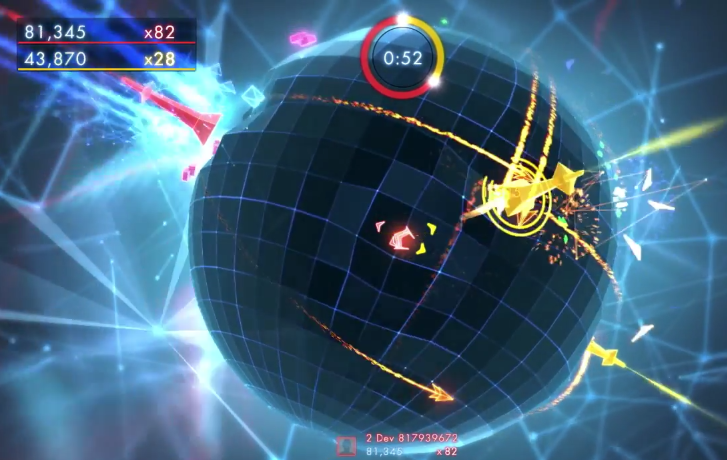
\includegraphics[width=150mm]{geometry_wars.png}
\caption{Geometry Wars: motivation for the game\label{overflow}}
\end{figure}

\section{Networking}
The networking for the game to function smoothly has to be fast non-blocking and Rigid (as game is deterministic).
\subsection{Salient features}
The Network structure will have the following salient features :-

\begin{itemize}
\item Networking will be implemented using UDP
\item A P2P lockstep model will be used to ensure synchronization.
\item how often packets are sent will be decided by the connection quality maximum being 10 times per second (after every 6 frames assuming 60 fps)
\item An acknowledgment protocol will be implemented to ensure distribution of all the data.
\item The network will be resilient to disconnection between peers. (as long as the network mesh forms a connected graph the game will go on)
\item In-case of disconnection the role of the player will be taken by a bot (computer)
\item A disconnected player will be allowed to reconnect to a game. The gamestate will be cumulatively sent to the reconnecting player.  
\item Multi-threading (4 threads per machine) will be implemented to maximize speed during synchronization
\item Player moves will be sent as data instead of game state to minimize data to be distributed. 

\end{itemize}
The networking process will be carried out in a different thread (with 4 sub-threads) from the "update game-state" and "draw" processes thus increasing efficiency and better synchronization rate.
\\
\\
\subsection{Problems and Solutions}
The main problems that we are expecting to come across are as follows.
\subsubsection{Packet Drop and Re-ordering}
In UDP packets are frequently dropped due to congestion and rerouting problems . We are going to solve this by encoding the packets with sequence numbers and implementing an acknowledgment protocol to ensure the complete distribution among all the peers.

\subsubsection{Disconnection between individual peers}
Problems arise when the connection between individual peers get disconnected.As a solution we are going to reroute the connection between those two individuals through one of the other peers.

\subsubsection{Variable Packet sending rate}
The connection may vary in quality during the games duration so if we use a lockstep model it will result in major latency in the frame rendering rate.As a solution we are going to setup another thread to regulate the packet communication rate based on the ping latency.



\section{Game engine}


\subsection{Graphics and rendering}

There are 2 primary things to be rendered:
\begin{itemize}
\item \textbf{Map} \\
The map will be a \textbf{3-D shape} which will be rendered in the form of a  \textbf{grid}. A number of squares will cover the surface of the map on which the players and the bullets will move. Inside each of the squares, there can be other objects that have to be rendered which are players, bullets and bots. The grid feature will make it easy to extend the game and make \textbf{different maps} because to make a new map, we just need to adjust the grid squares in their new positions.
\item \textbf{Players, Neutral bots and Bullets} \\
The players will be rendered as simple \textbf{geometrical shapes} such as a polygon which will be shaded accordingly so that the user can know where the player is heading currently.\\
The current player will always appear at the center of the screen. When the player moves in the game, the \textbf{map being rendered to this player will rotate} in the opposite direction so as to give the visual effect of the movement of the player.\\
However, the position of other players, neutral bots and bullets on the rendered frame will depend on which grid they currently lie in.\\
\end{itemize}
\textbf{OpenGL implementations idea:}\\
The map as such will remain at a fixed position in terms of coordinates however the camera focusing on the map will move and rotate around the map to give a visual effect of a rotating map.\\
The properties of the camera (position, aim, rotational angle) will be determined by the position and the direction in which player is facing at that moment. 
\begin{itemize}
\item The position being at the line joining center of map to player and at a fixed distance from the player.
\item The aim being the player.
\item The rotational angle being along the direction where the player is currently heading.
\end{itemize}
\subsection{Physics}

The physics would include primarily using the data structures of the players,bots, and bullets for consideration of the following:-

\begin{enumerate}
\item Determine the motion of the players:\\
All the information about the player motion would be packed in a data  structure. It would contain the following:-
\begin{itemize}
\item Position on the grid.
\item Velocity
\item Objects in the bounding region defined for that player

\end{itemize}

\item Determine the motion of the bots:
The motion of the bots will be governed by the AI implementation of the game. It would vary across difficulty level of the game. As an instance of this, the bounding region for a bot which is related to its reaction to the state of the game will vary for different levels. 
\item Determine trajectory of the bullets and other damage inflicting objects:
All the damage inflicting objects available as weaponry for a player has its own dynamics. For example a bullet shot will be different to an EMP wave attack.
\item Detecting collisions between the different elements in play:\\
This would make use of the motion details of the colliding bodies. This case also accounts for collision between a player/bot with a damage inflicting object.


\end {enumerate}


\subsection{Artificial Intelligence}
The AI component of the program will take the following points into consideration:-\\
\begin{itemize}
\item The AI implementation will be based on a finite state machine.
\item There will be many states like defensive, moderate, idle, aggressive, sacrificial, protective modes,etc. 
\item There will be various parameters that will affect the current state and state transition like Current Health, Current power up, Allies and Enemies visible (their power ups, health, kill streak), Bullets approaching (how many?, powered up bullets?).
\item Depending on the above parameters FSM would be made for the bot control. FSM will have all the possible states and depending on the latest parameters received, there would be a state transition for the object in consideration.
\item The transition will also be much efficient and will provide a better game-play with increasing difficulty. The FSM would be different with each varying difficulty.
\item For a bot team the AI will include various tactical parameters like protecting the killing streak, kill for kill for more points, etc.
\item Since all the machines would be in real time synchronization each of them will calculate the next position of each bot and render them on the screen.
\item Also having same algorithms for each machine the sequence of decision taken by each bot will be same for all machines and hence they will remain in sync for the next cycle.
\item At the end of cycle for each bot various keyboard output equivalent to that sent by a human will be forwarded if necessary to other systems by networking.
\item AI programming for neural bots will be a bit different from normal bots. They will primarily attack those unit(of either team) that is in their respective vision.
\item The main aim of neutral bots will be to attack any unit in vision (irrespective of the unit's parameters) rather than killing a particular target. Their FSM would be simpler as they would have less states(variation in playing style) than team bots.
\end{itemize}


\section{Debugging with work flow}

For debugging based on the current work flow, our approach is to break the development process into independent components. This would be the first stage of testing:-
debugging networking with threads implementation, rendering , physics of the objects,etc. Then we would integrate all of these and work on the resulting issues.  

\end{document}